Following the phenomenological study~\cite{Ilten:2017rbd}, four key variables characterizing the \gbb process are measured:
\begin{enumerate}
\item angular distance between $b\bar b$: $\drbb = \sqrt{ \Delta(b,b)^2+\Delta \eta(b,b)^2 }$,
\item momentum sharing: $\zpt = \frac{ p_{\text{T},2} }{ p_{\text{T},1}+p_{\text{T},2} }$, where $p_{\text{T},1}$ and $p_{\text{T},2}$ are the \pt of the leading and sub-leading $b$'s
\item dimensionless mass: \mpt where $m$ and \pt are the mass and transverse momentum of the sum of four-vectors of the $b$'s
\item angle between production and splitting plane of the gluon: \dphi
\end{enumerate}

The distributions of these variables in the truth level are shown in Figures~\ref{fig:gbb-gbbdistributions} and \ref{fig:gbb-gbbangle} as predicted by \textsc{Pythia8}. While the first three variables are sensitive to variations in fragmentation modeling up to 10$\%$, the \dphi variable is sensitive to the choice of gluon spin. 



\begin{figure}[htpb!]
\begin{center}
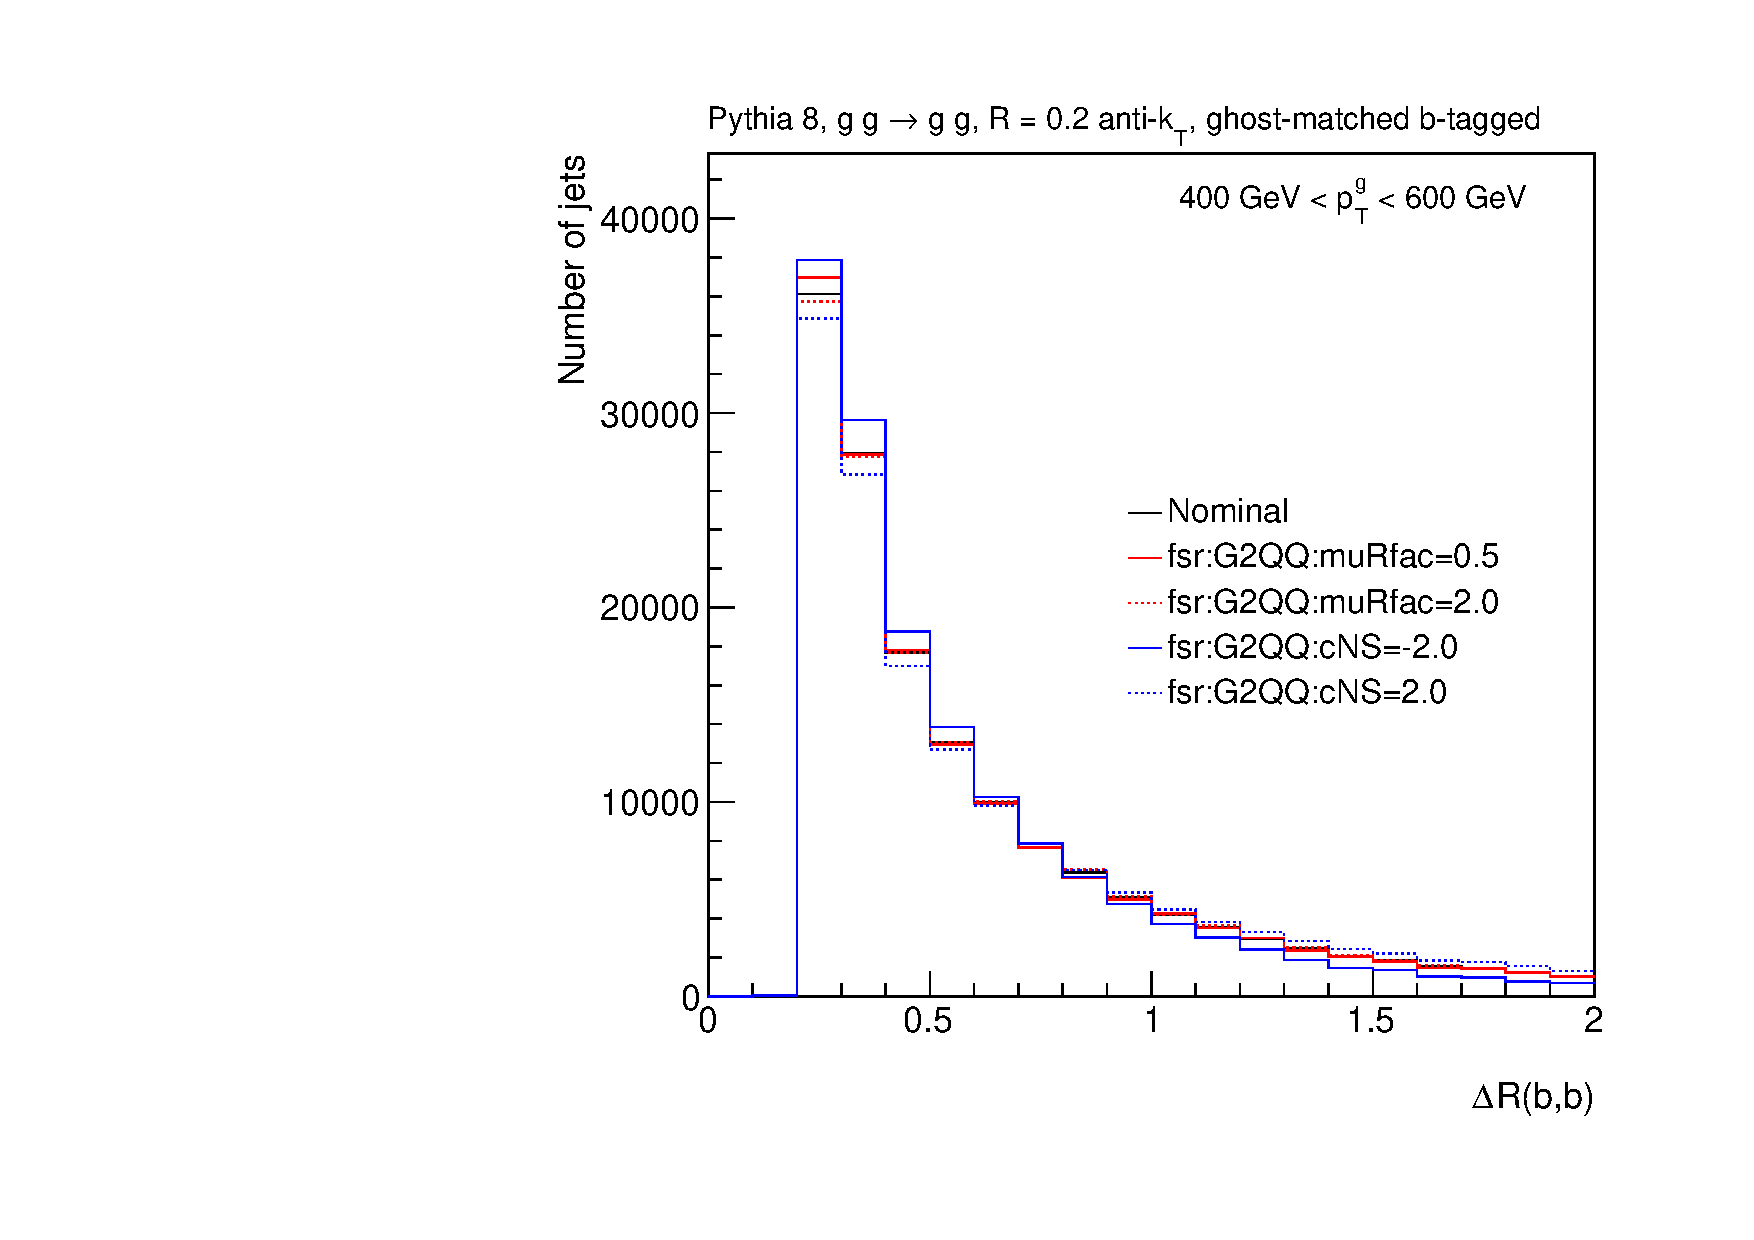
\includegraphics[width=0.33\linewidth]{figures/gbb/truth_level/DeltaRbb.pdf}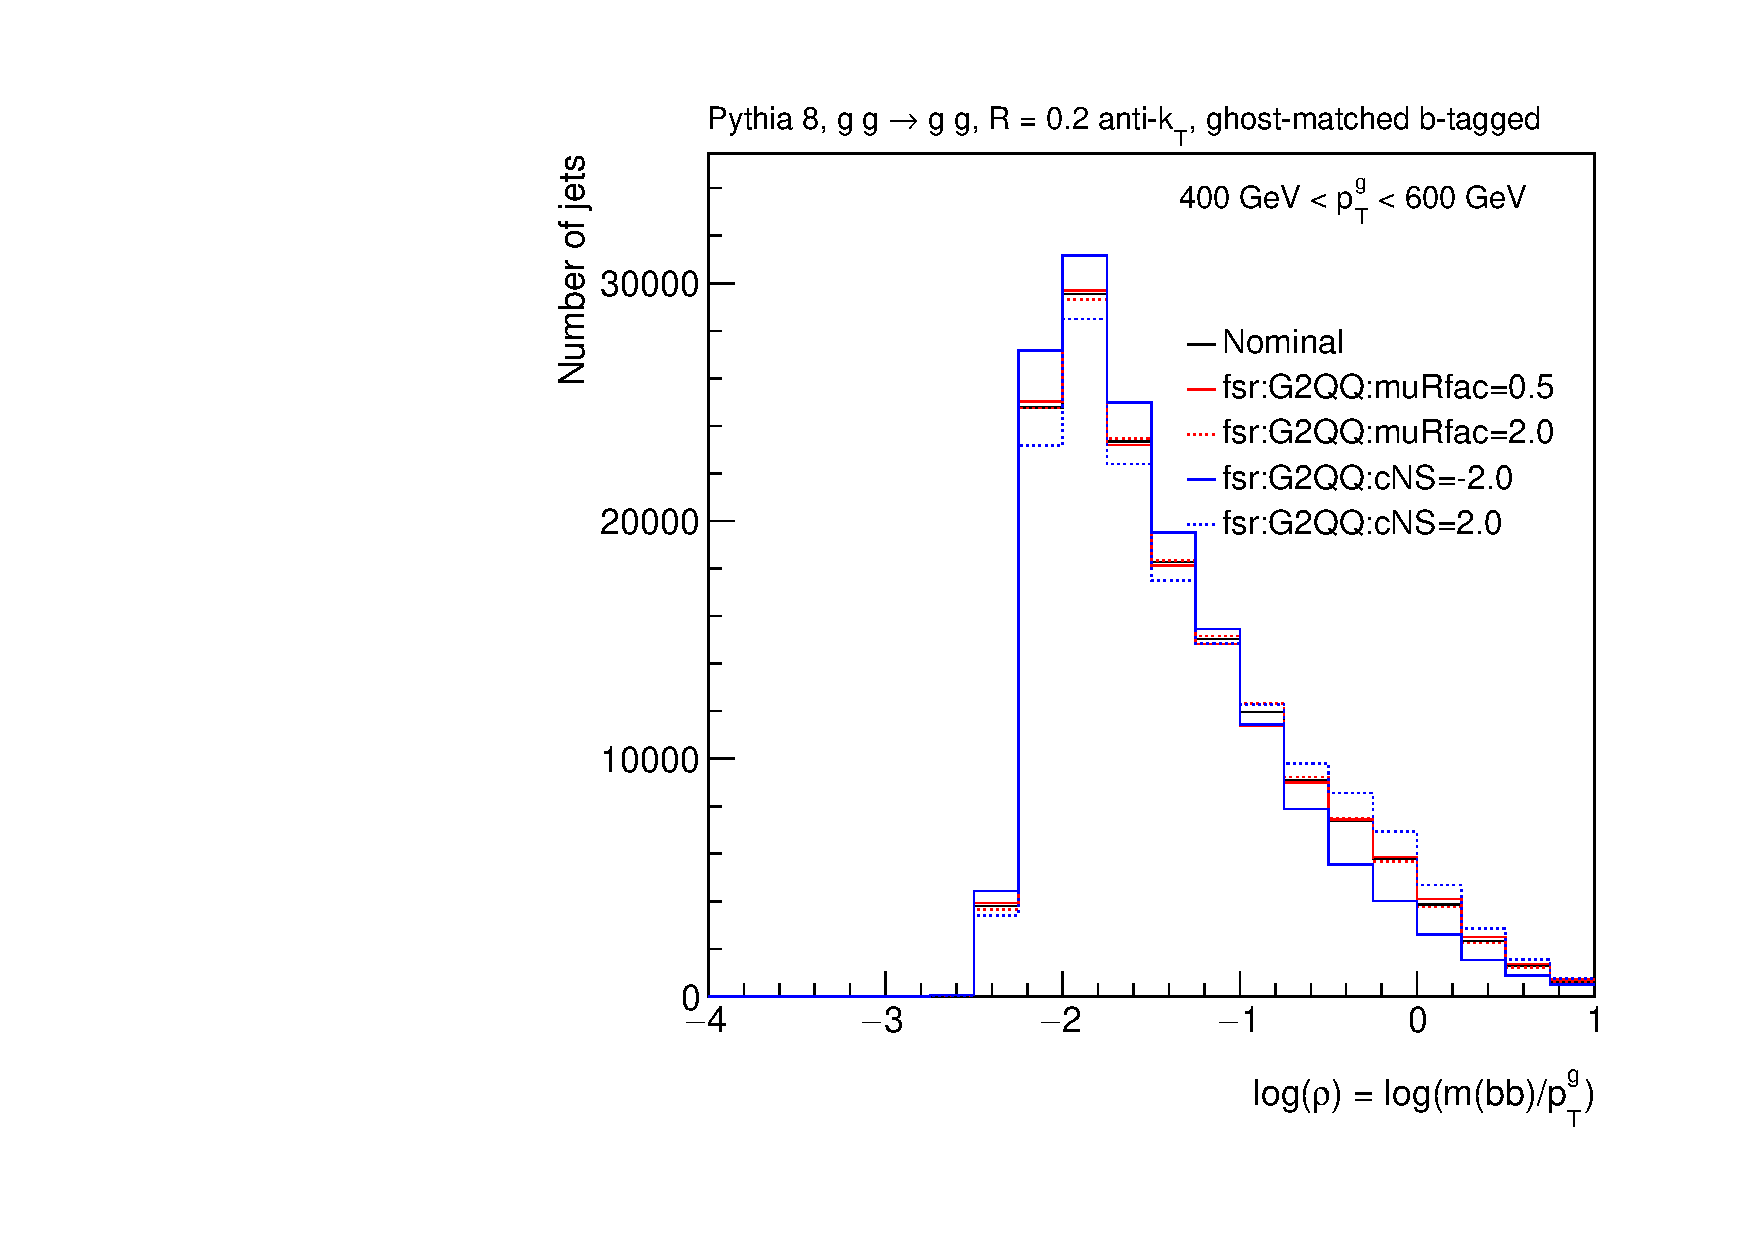
\includegraphics[width=0.33\linewidth]{figures/gbb/truth_level/rhobb.pdf}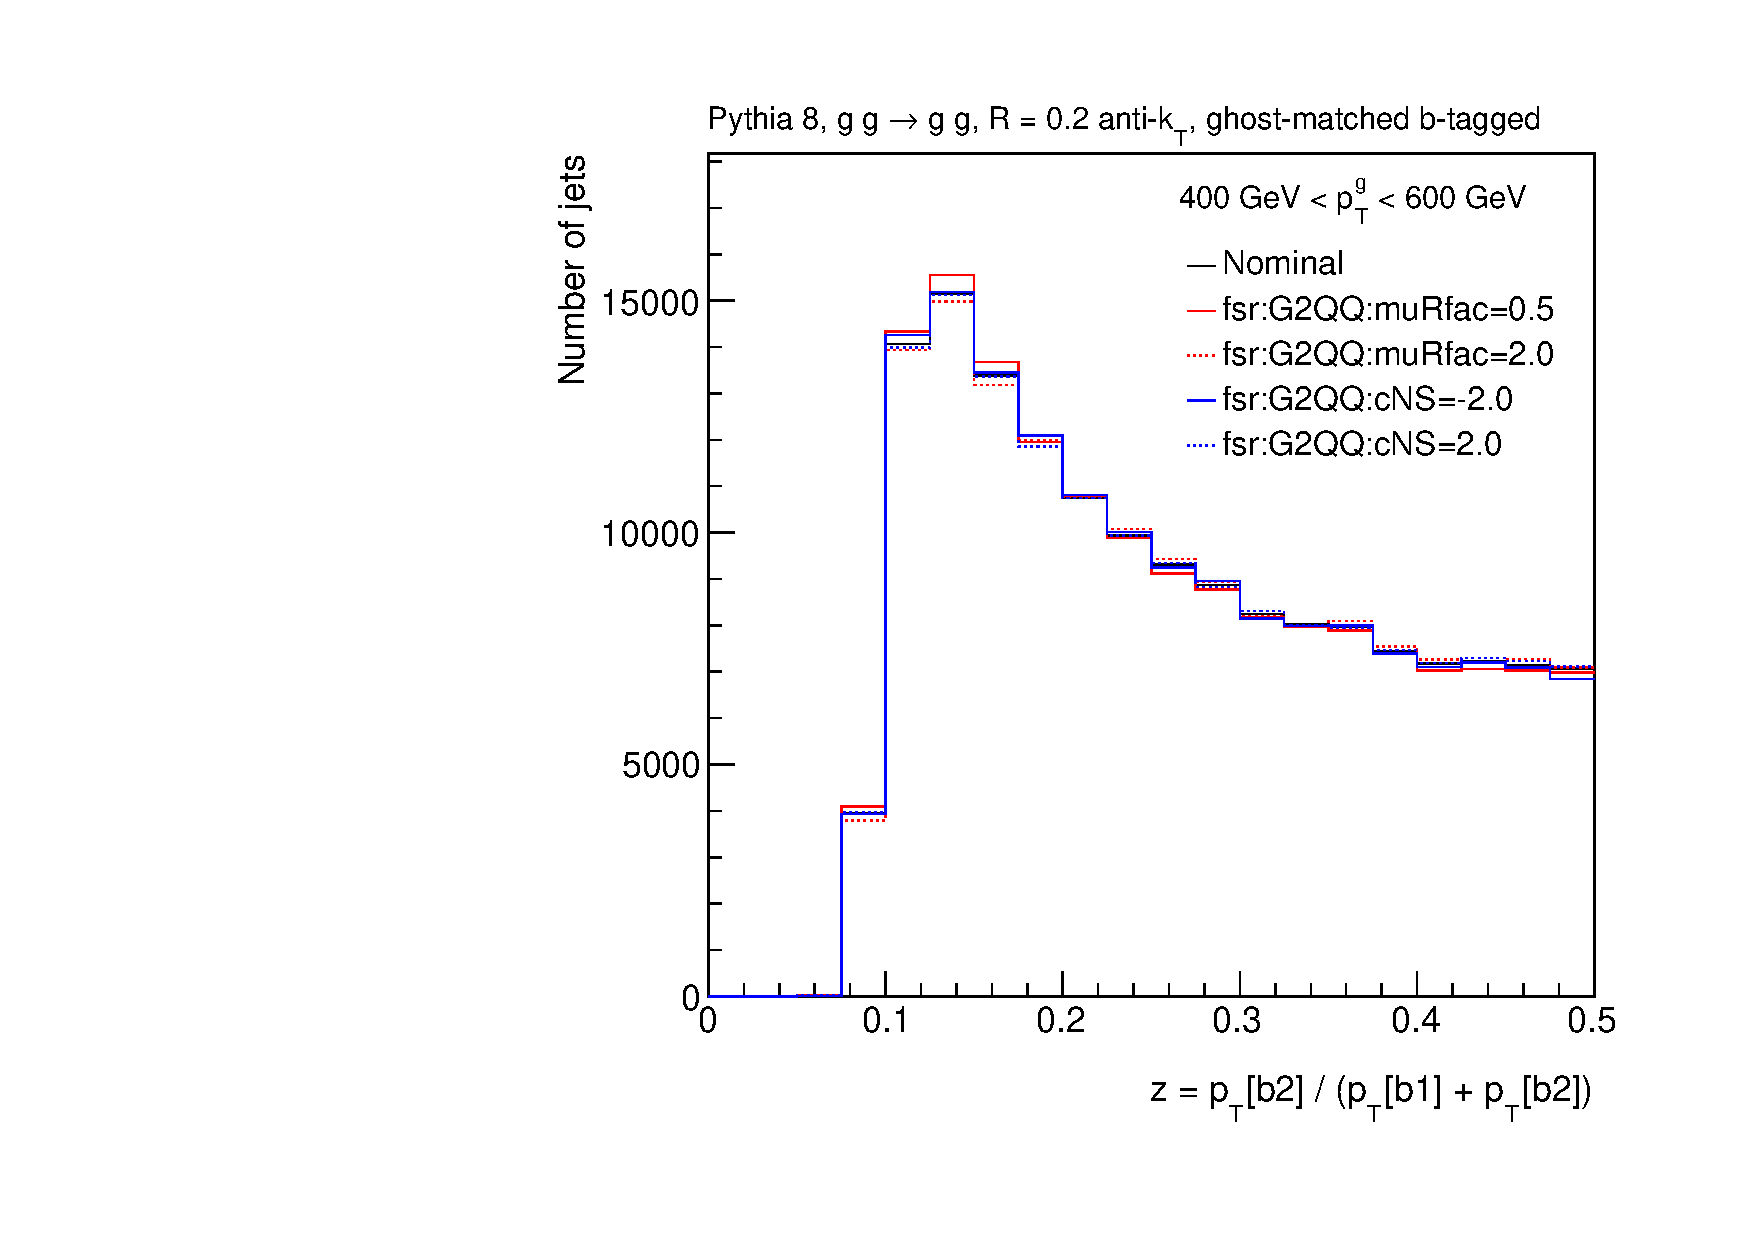
\includegraphics[width=0.33\linewidth]{figures/gbb/truth_level/DeltaZbb.pdf}
\caption{The distributions of $\drbb, \mpt$, and $\zpt$ in simulation along with a series of variations in the form of the fragmentation described by Pythia~\cite{pythiavariations}.} 
\label{fig:gbb-gbbdistributions}
\end{center}
\end{figure}

%\begin{figure}[htpb!]
%\begin{center}
%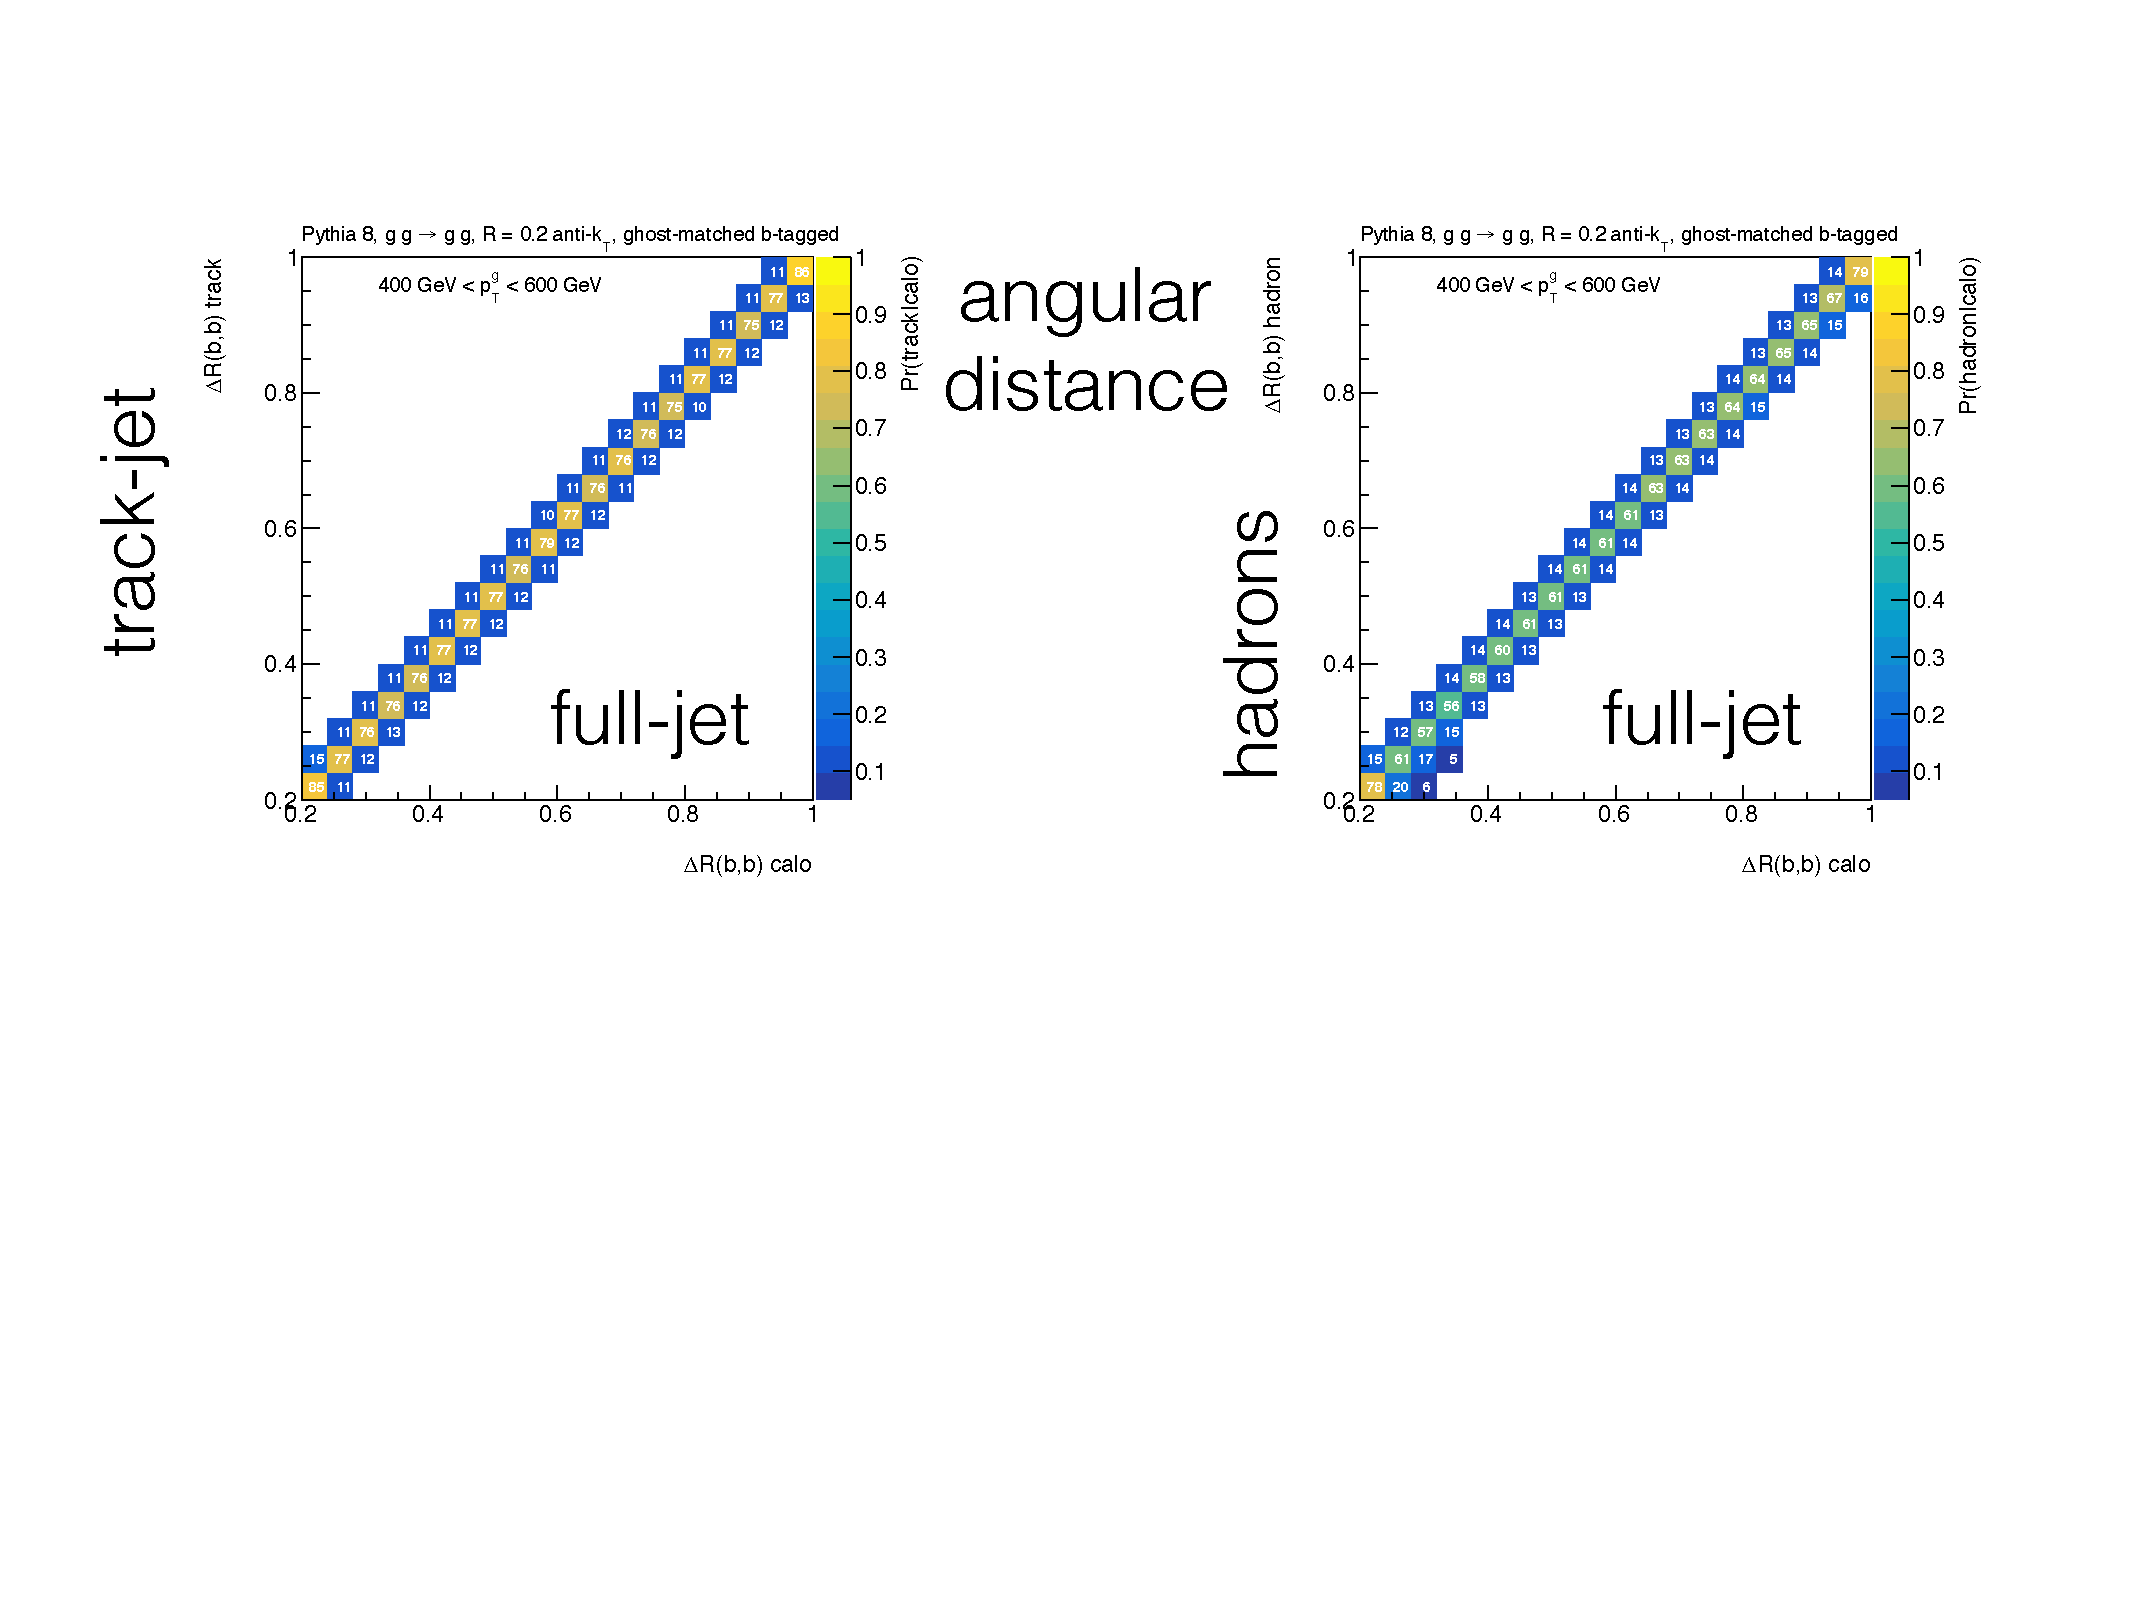
\includegraphics[width=0.95\linewidth]{figures/gbb/truth_level/compare2.pdf}\\
%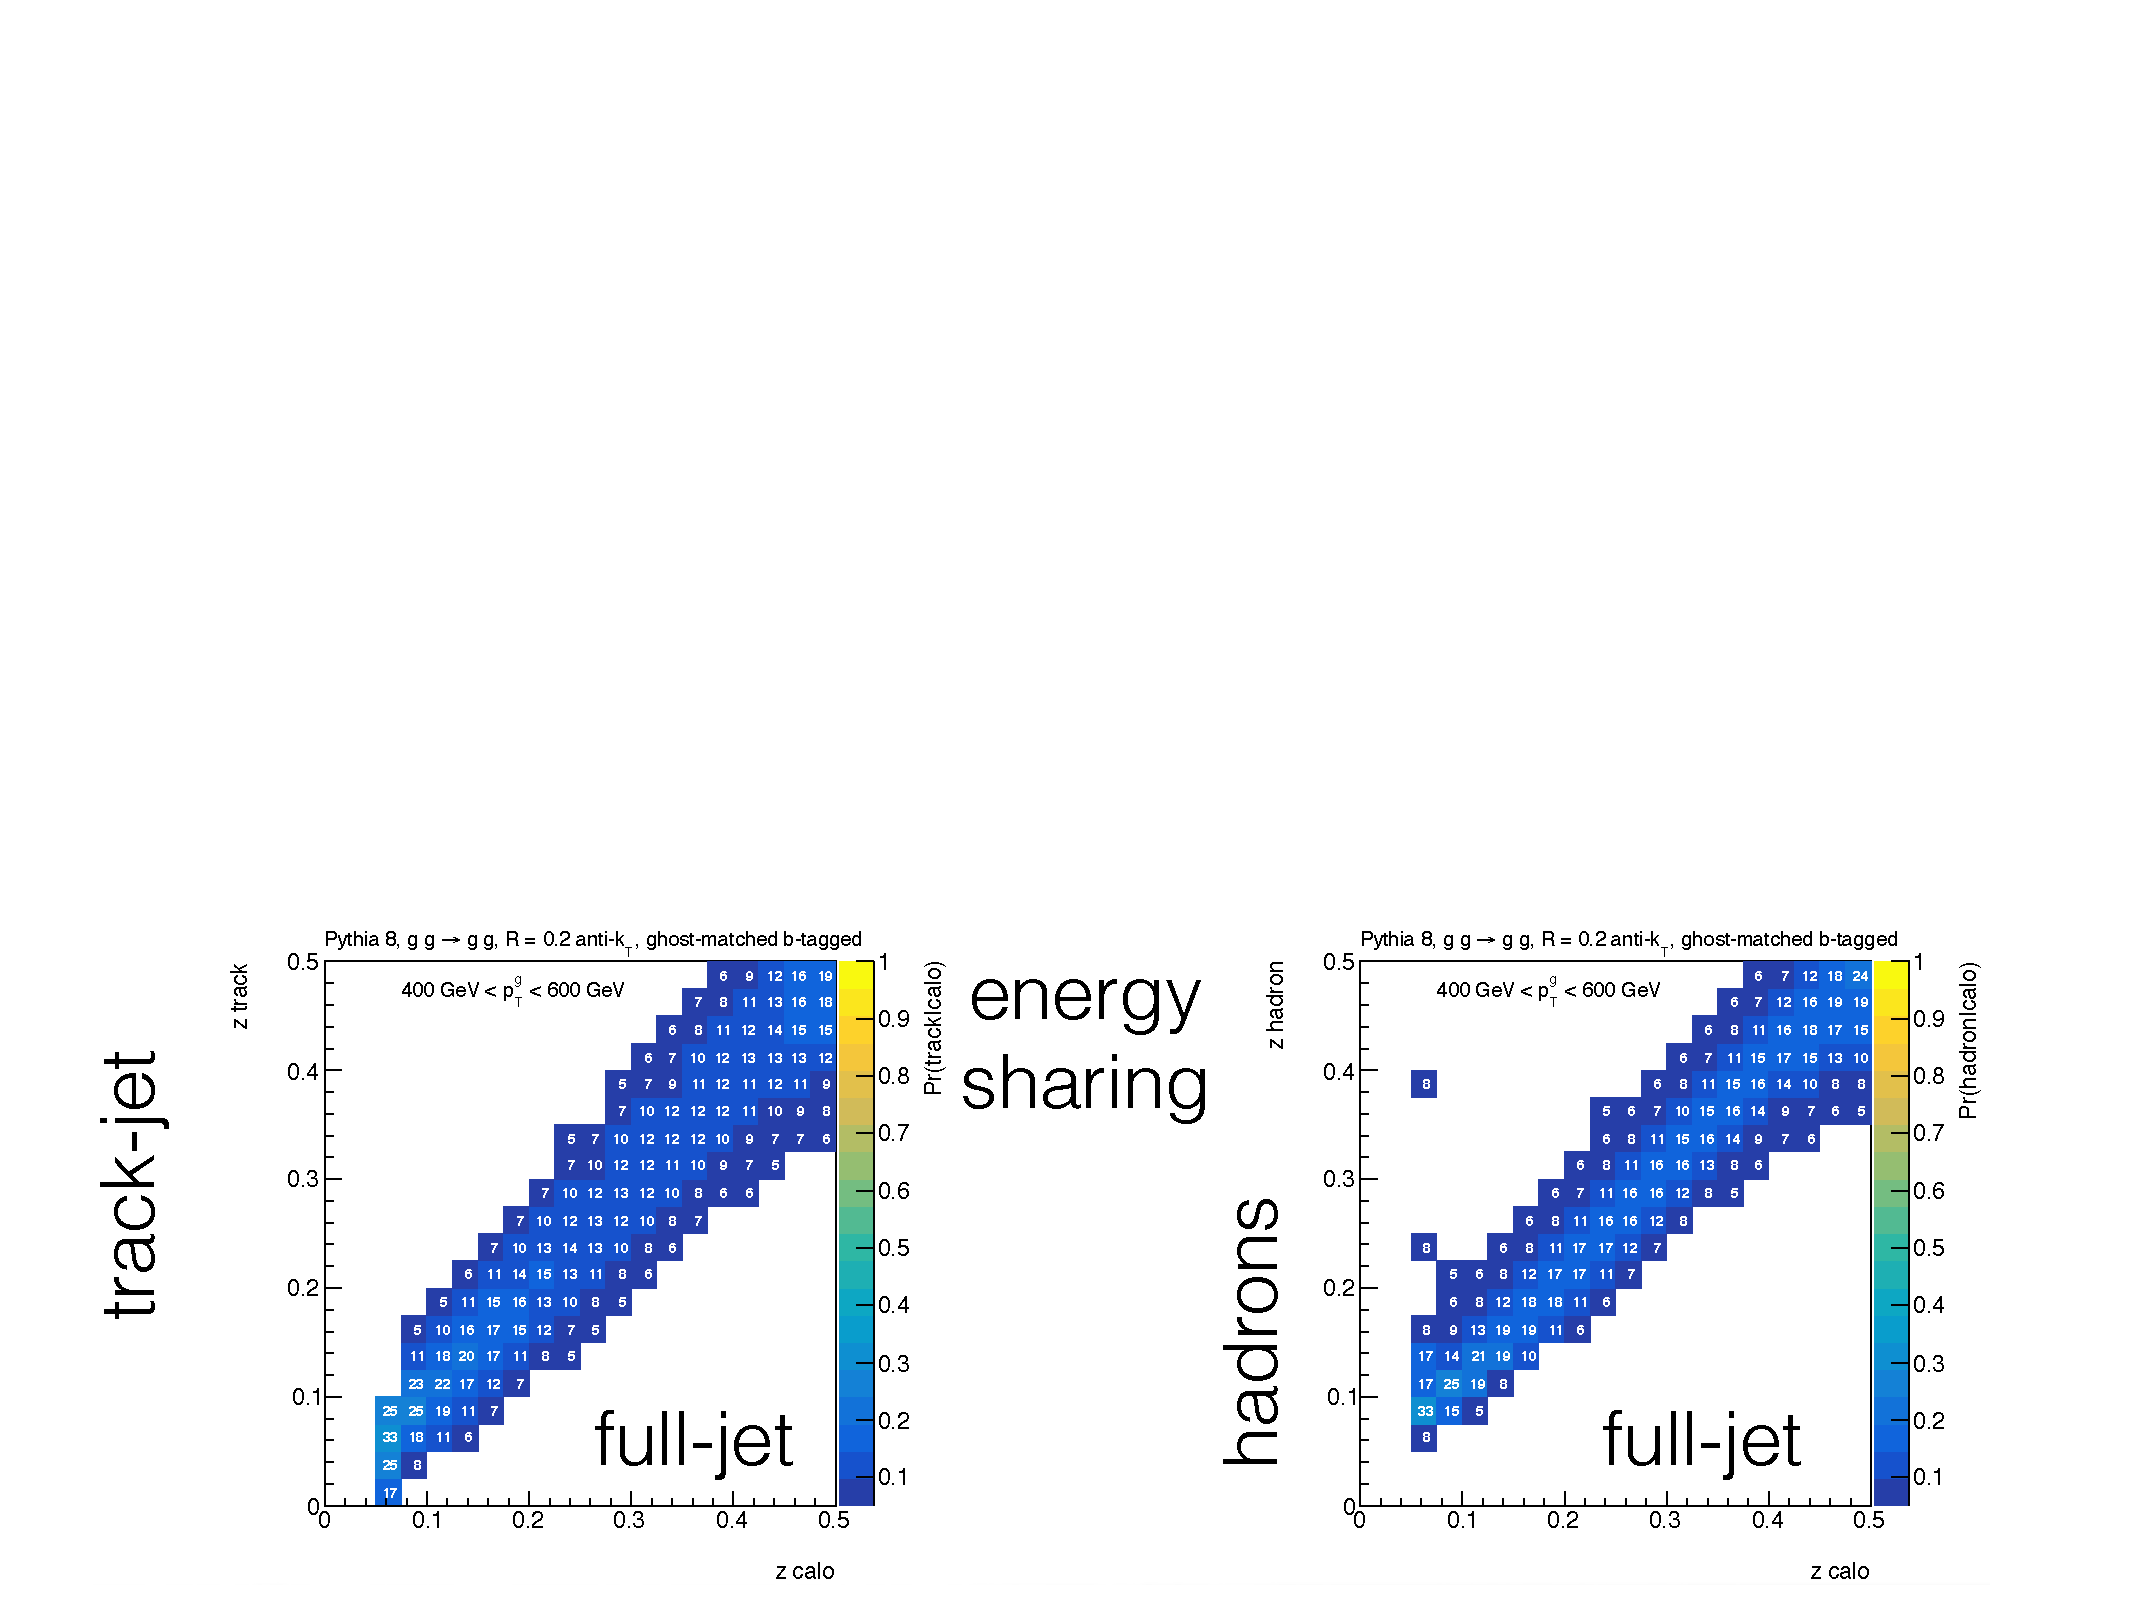
\includegraphics[width=0.95\linewidth]{figures/gbb/truth_level/compare1.pdf}
%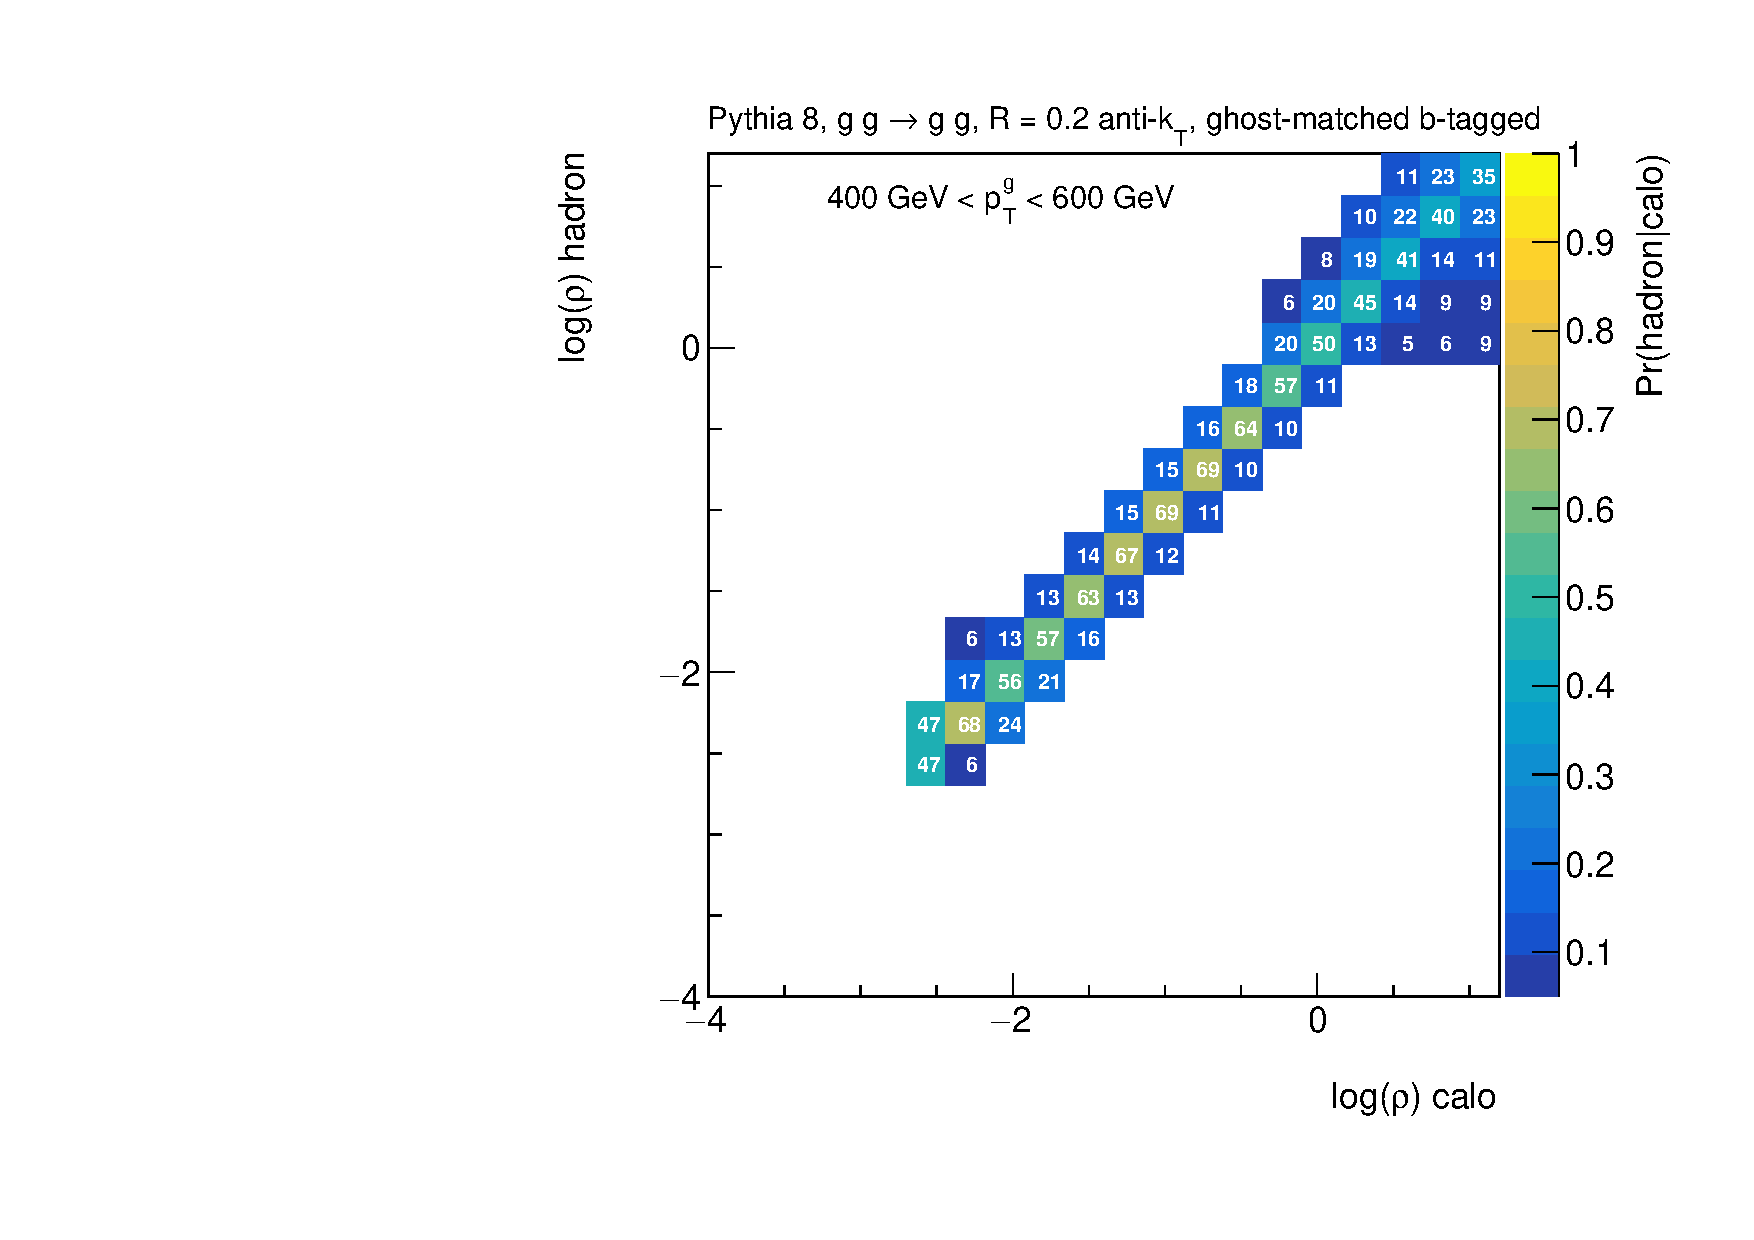
\includegraphics[width=0.45\linewidth]{figures/gbb/truth_level/rho_calo_track_b.pdf}
%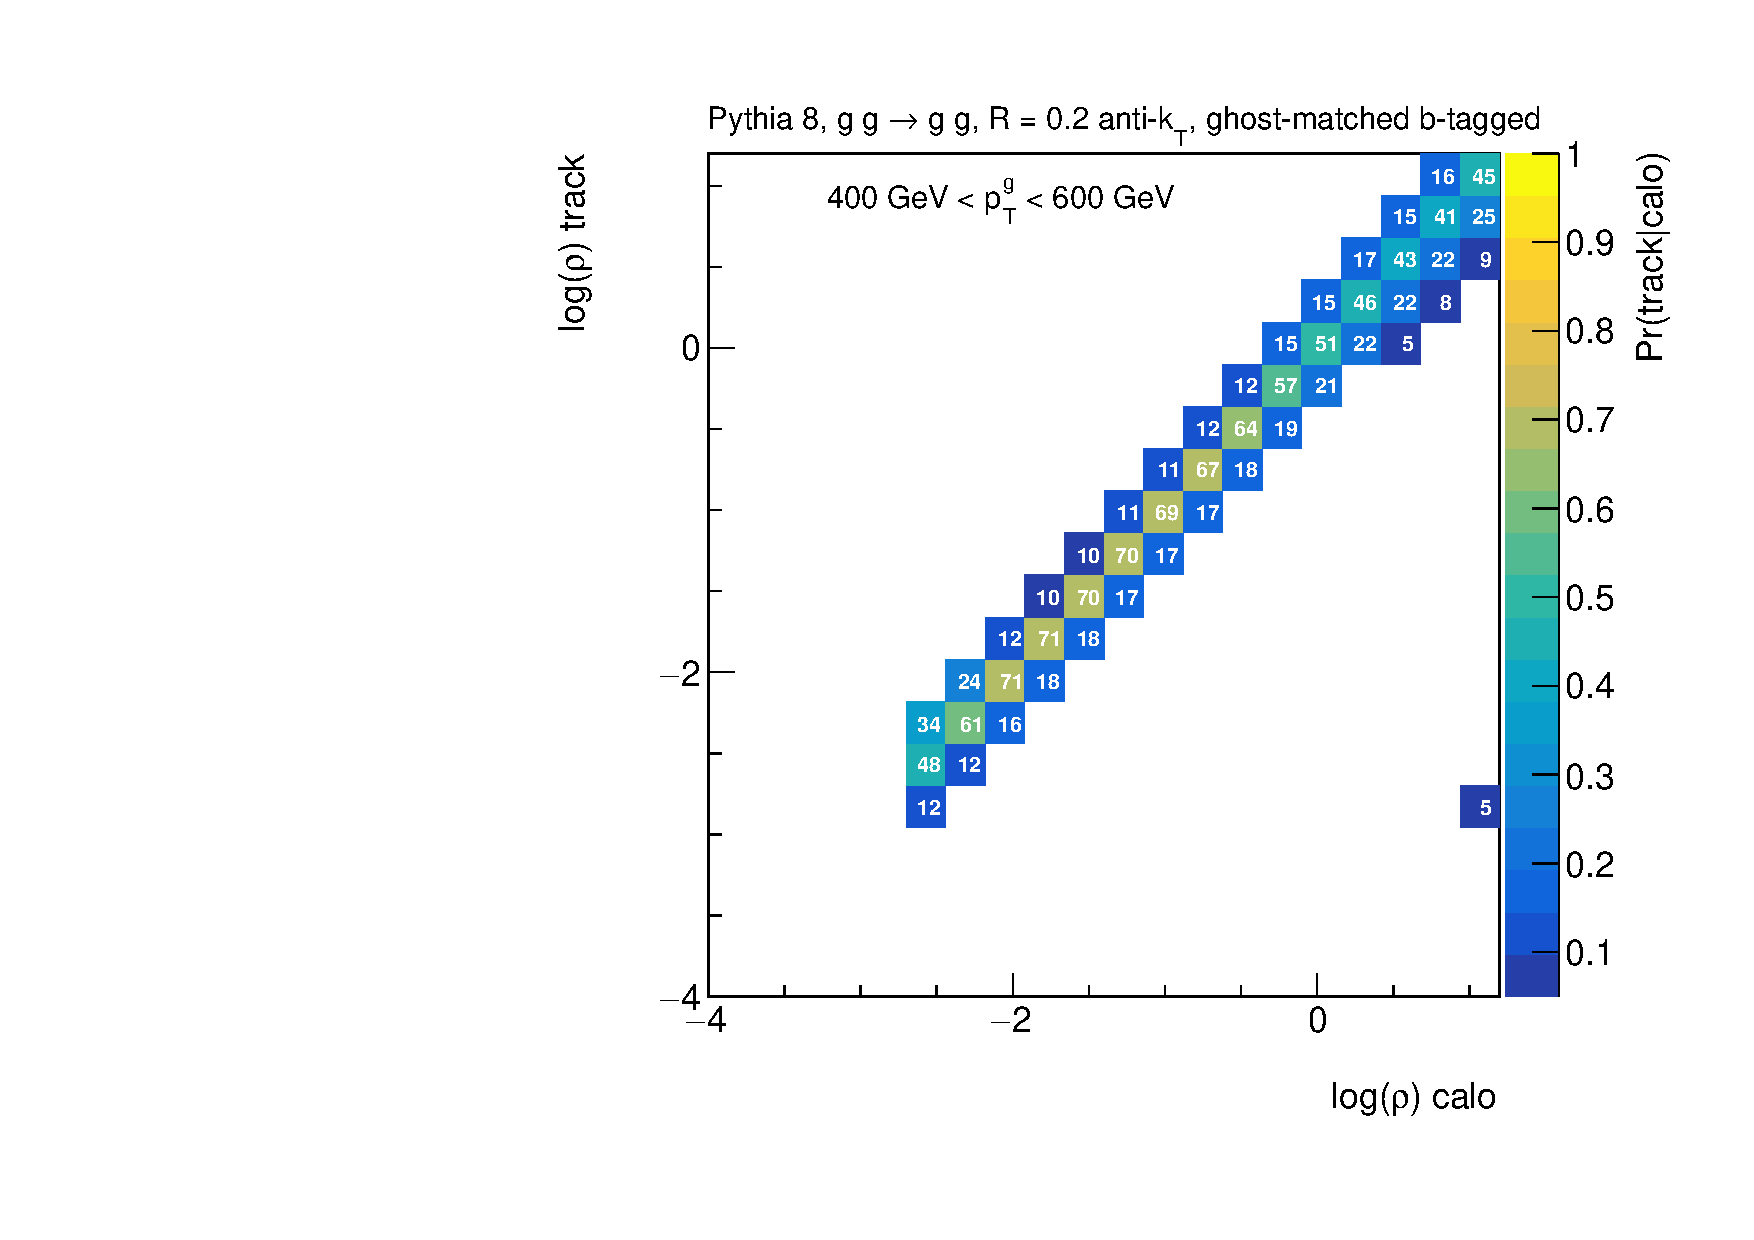
\includegraphics[width=0.45\linewidth]{figures/gbb/truth_level/rho_calo_track.pdf}
%\caption{The two-dimensional distribution of two of the variables from Fig.~\ref{fig:gbb-gbbdistributions}, but using different definitions of `b' ($B$-hadrons, $b$-jets, $b$-track-jets).} 
%\label{fig:gbb-gbbresponse}
%\end{center}
%\end{figure}

\begin{figure}[htpb!]
\begin{center}
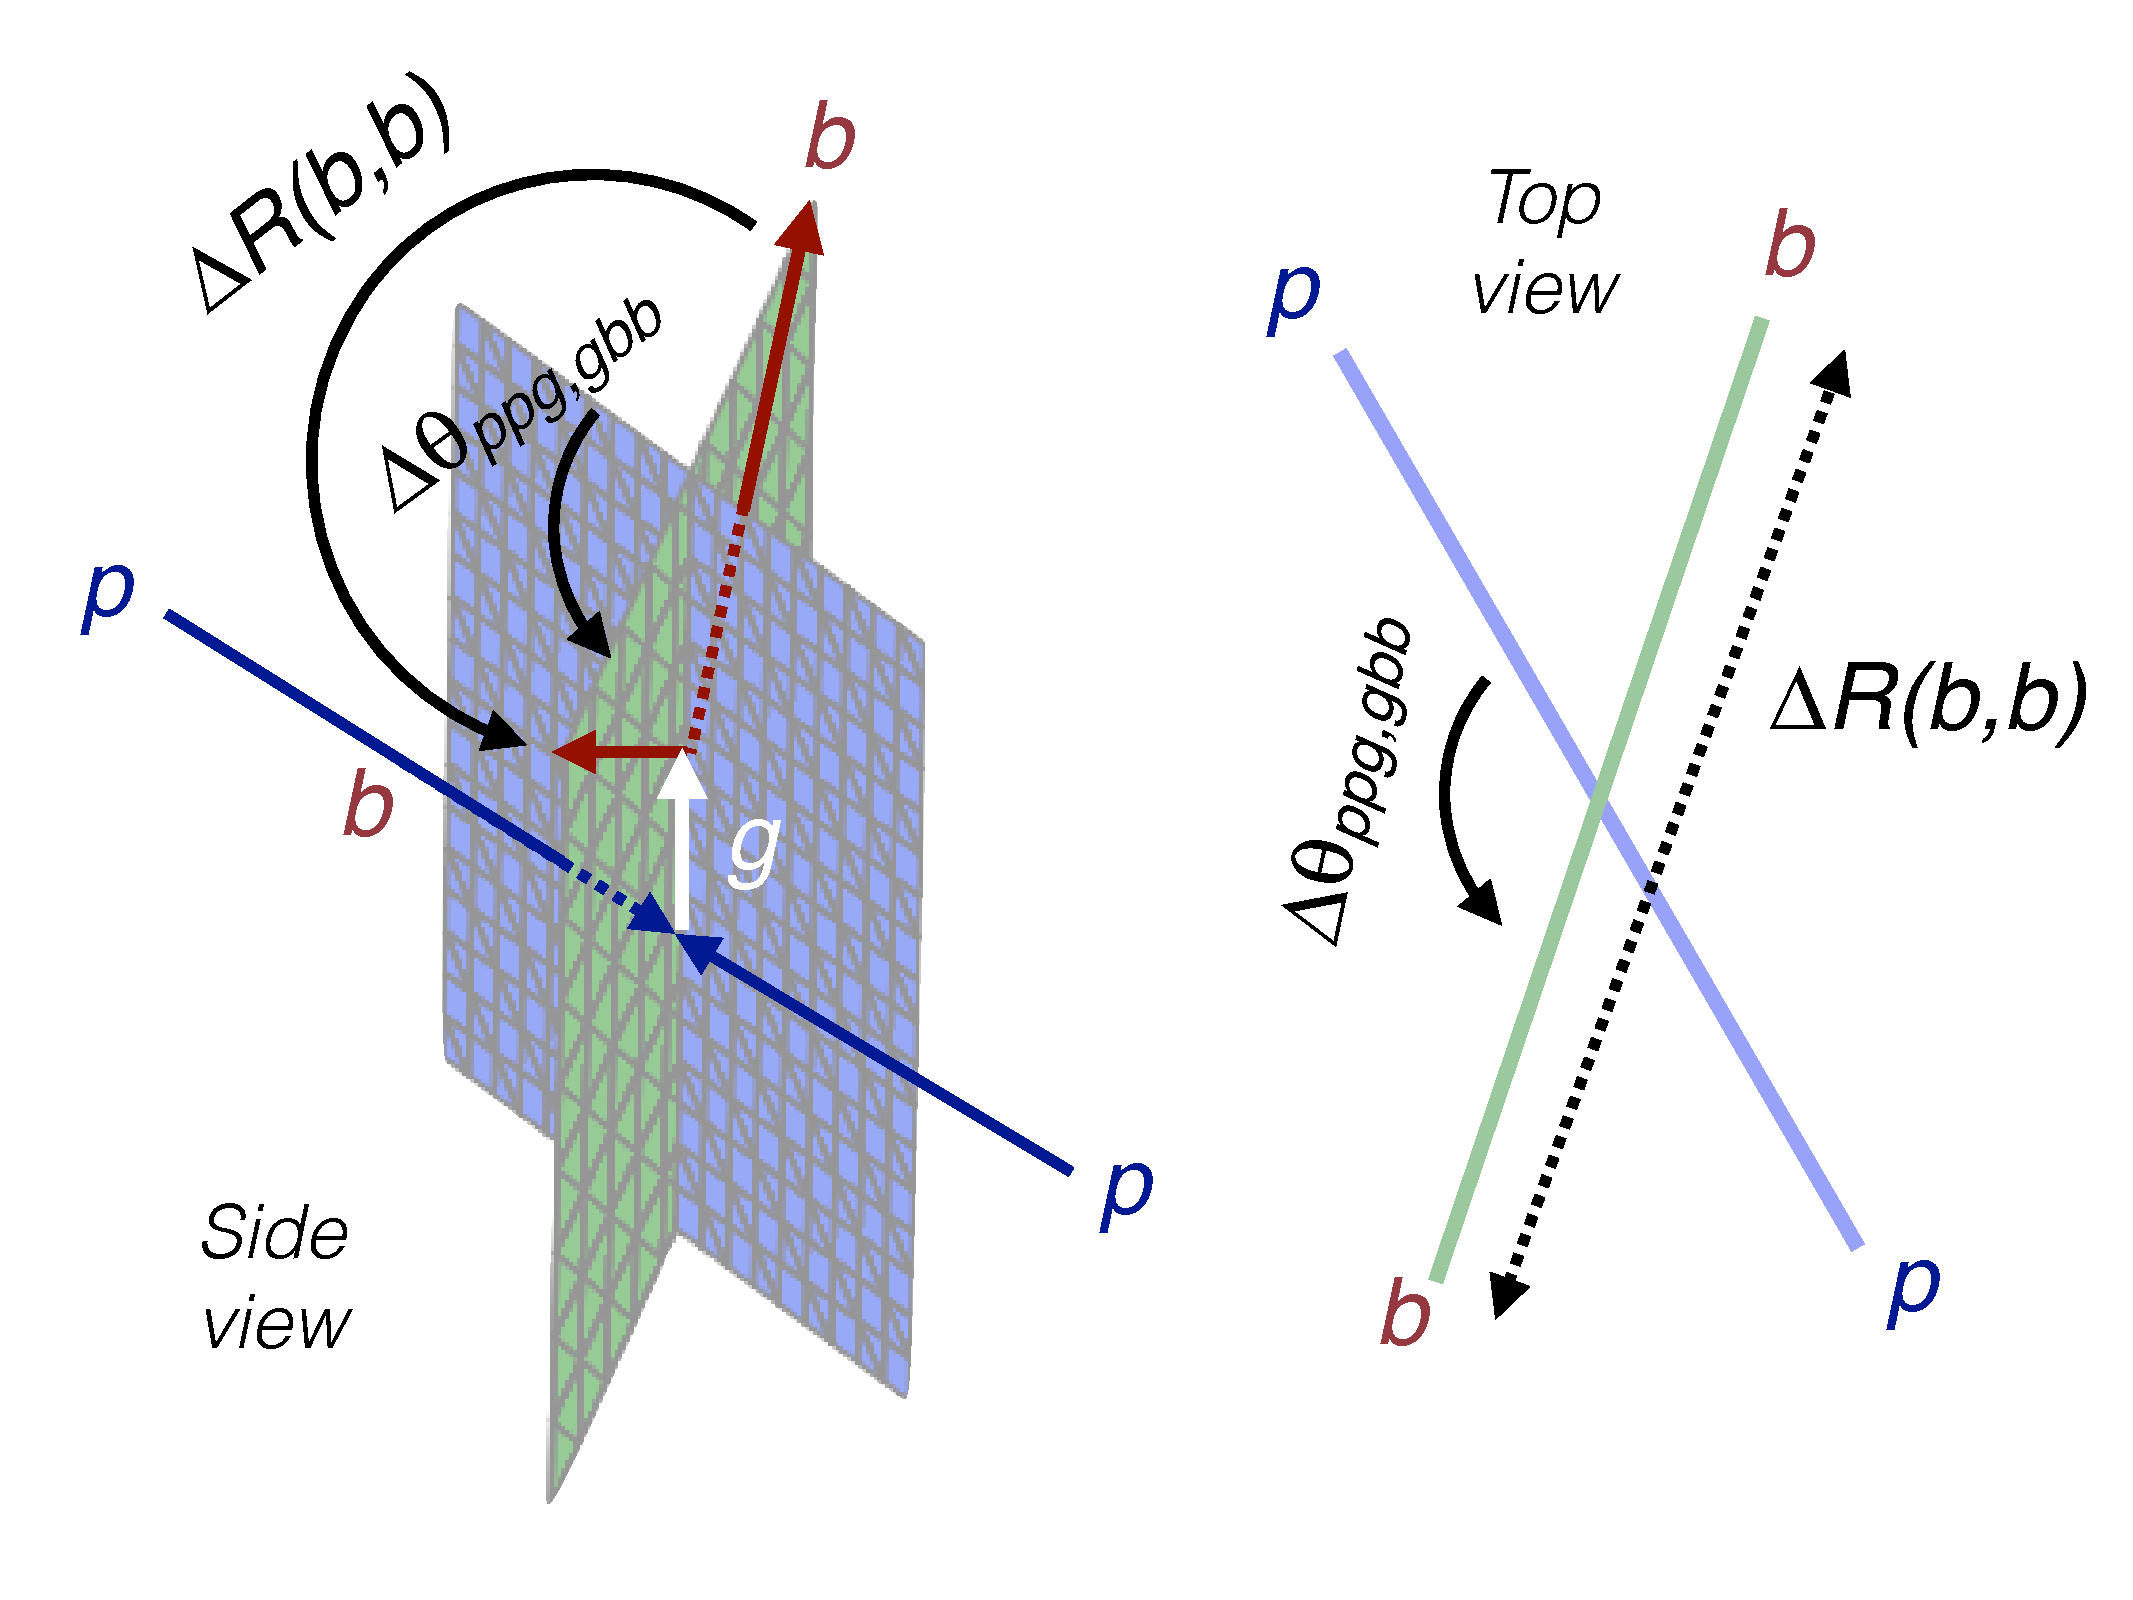
\includegraphics[width=0.45\linewidth]{figures/gbb/schematic.pdf}
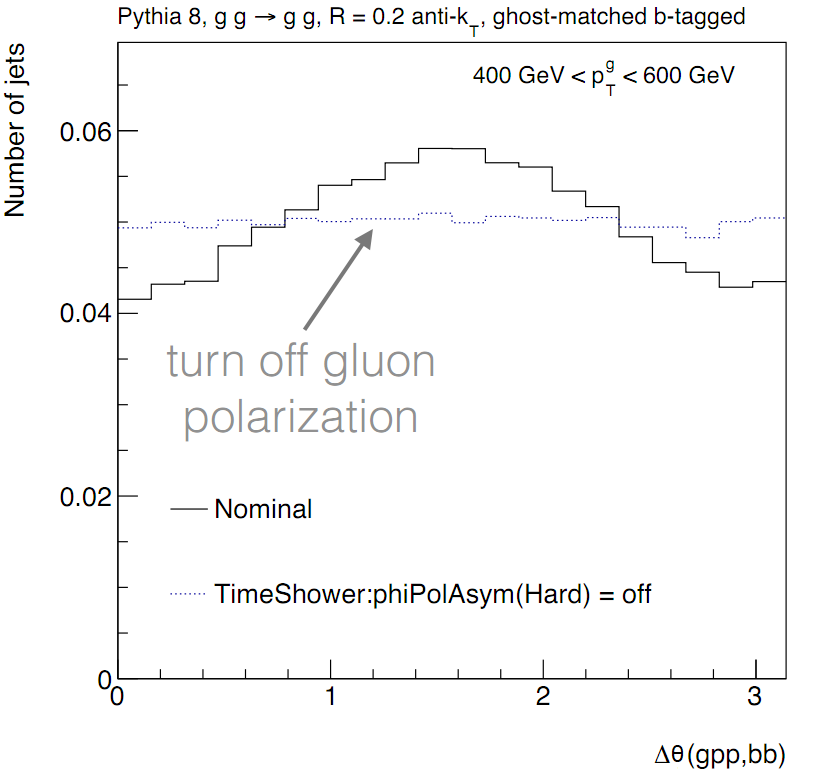
\includegraphics[width=0.45\linewidth]{figures/gbb/dtheta.png}
\caption{The angle $\Delta \theta$ that the $g\rightarrow b\bar{b}$ plane makes with respect to the $pp\rightarrow g$ plane. This distribution is sensitive to the gluon polarization choice.} 
\label{fig:gbb-gbbangle}
\end{center}
\end{figure}


All the reconstructed distributions are eventually unfolded to truth level. One has the options of unfolding the reconstructed distributions to $b$-quarks, $b$-hadrons and $b$ truth jets with the last option being easiest. As will be covered in Sec.\ref{sec:gbb-obj}, since this analysis uses track jets to be proxies of the $b$-quarks and the angular resolution of track jets are very good, the truth angular variables shall have very low bin migrations between the choice of $b$-quarks and truth $b$ track jets. To avoid the trouble of reconstructing $b$-hadrons and $b$-quarks, which depend on the modeling of hadronization, the analysis hence unfold the reconstructed distributions to truth $b$ track jets. 
